\begin{frame}
	\frametitle{Benes Network}
	\begin{center}
		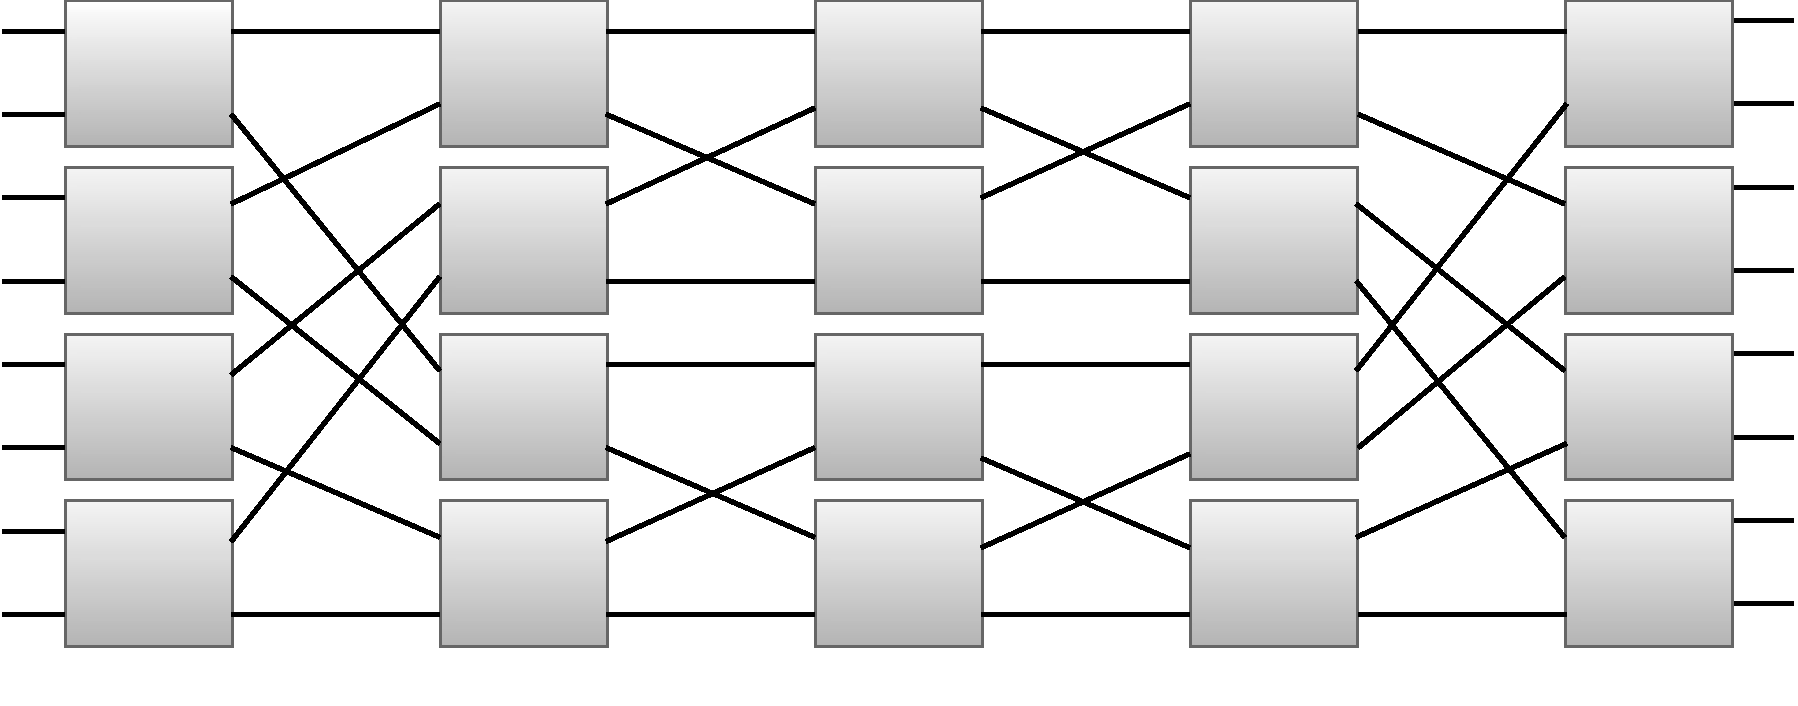
\includegraphics[width=0.9\linewidth]{benes_network.pdf}
	\end{center}
\end{frame}

\begin{frame}
	\frametitle{Benes Network: Recursion}
	\begin{center}
		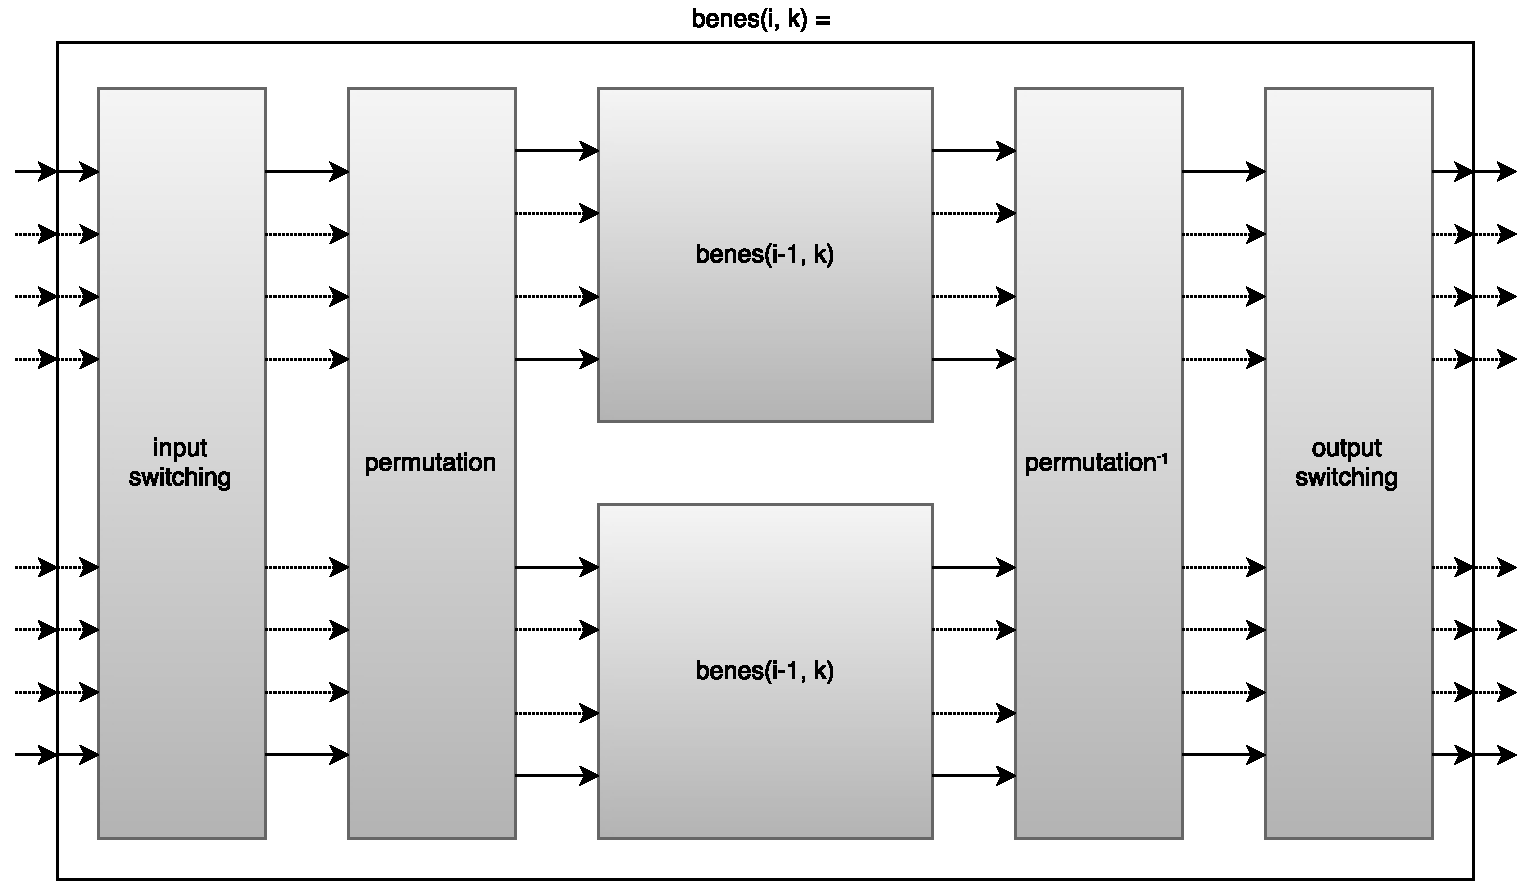
\includegraphics[width=0.9\linewidth]{benes_recursion.pdf}
	\end{center}
\end{frame}

\begin{frame}
	\frametitle{Benes Network: Banyan Stalling Switch}
	\begin{center}
		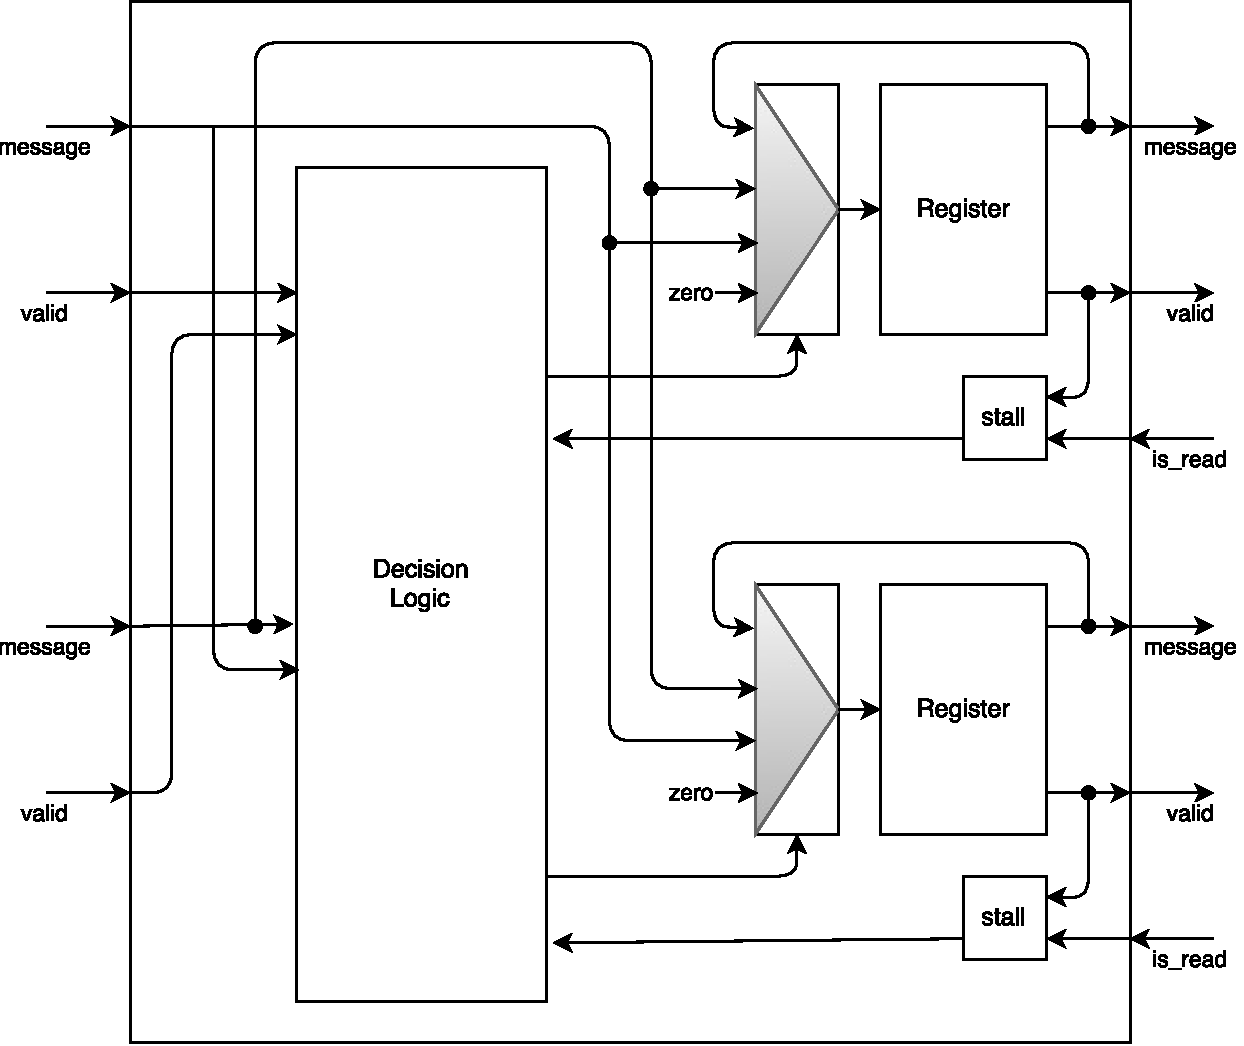
\includegraphics[width=0.7\linewidth]{banyan_stall_switch.pdf}
	\end{center}
	\begin{itemize}
		\item Fixed route for each packet, based on bit $k - i$.
	\end{itemize}
\end{frame}
	
\begin{frame}
	\frametitle{Benes Network: Companions}
	\begin{center}
		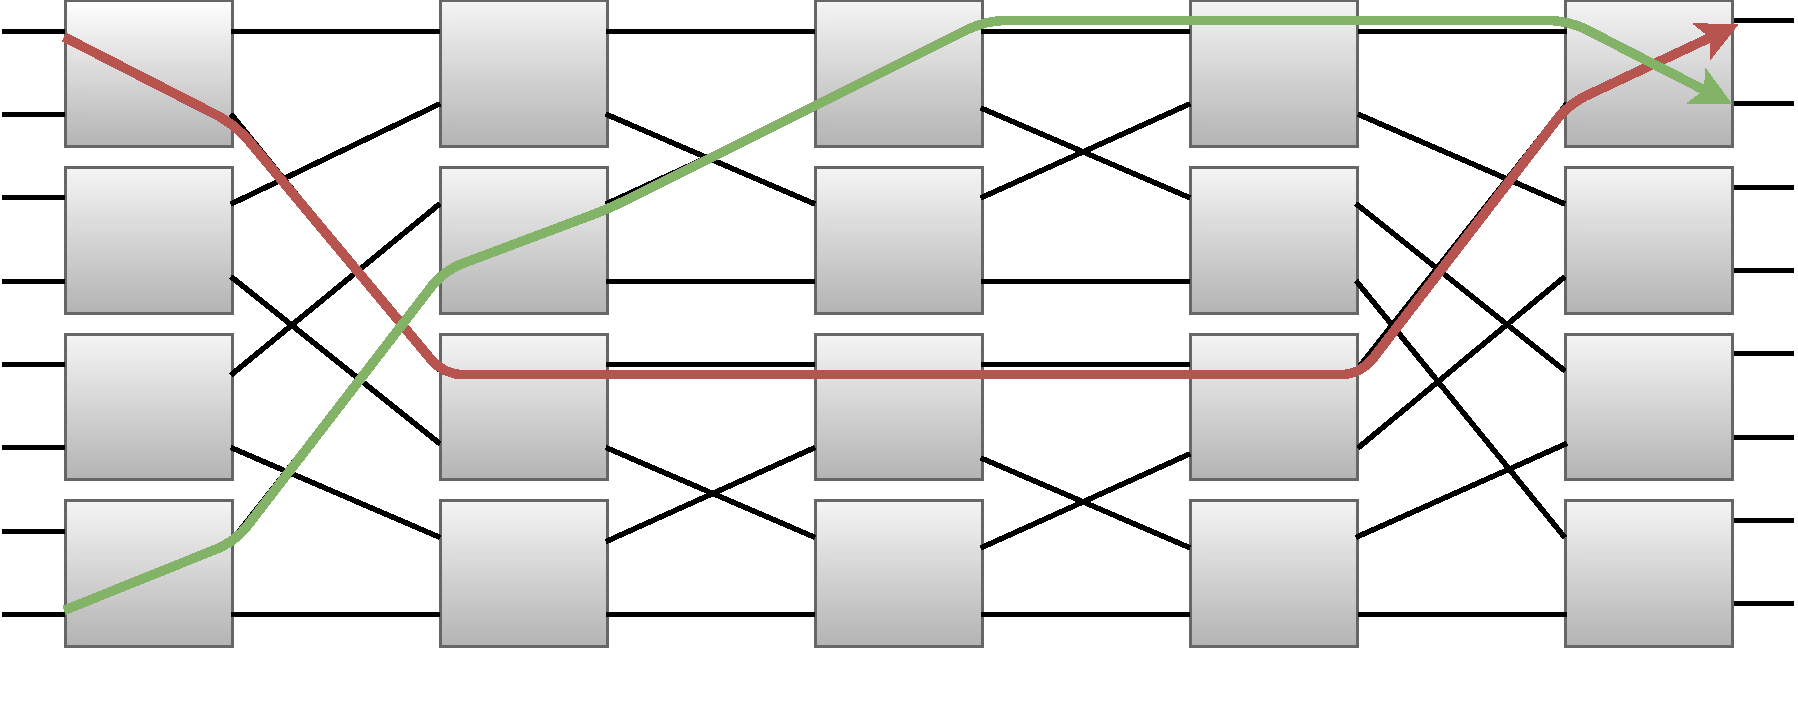
\includegraphics[width=0.9\linewidth]{benes_companions.pdf}
	\end{center}
	\begin{itemize}
		\item Concept by Tripti
	\end{itemize}
\end{frame}

\begin{frame}
	\frametitle{Benes Network: Input Column}
	\begin{center}
		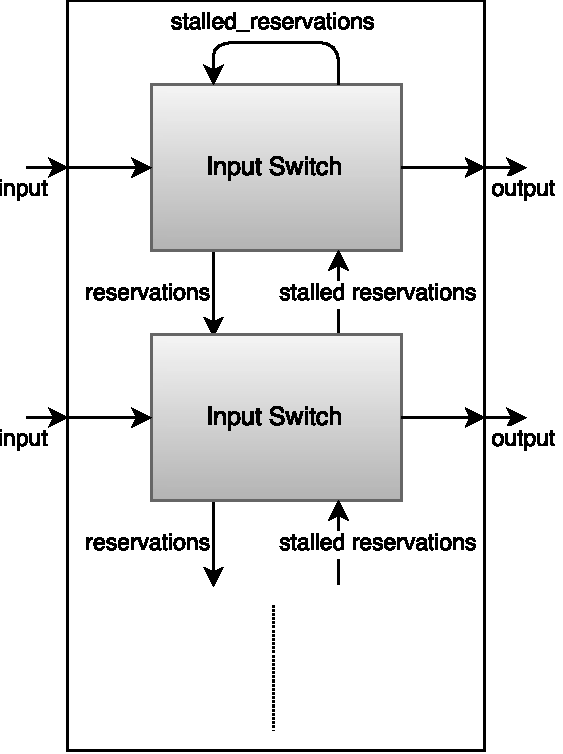
\includegraphics[width=0.3\linewidth]{benes_input_column.pdf}
	\end{center}
	\begin{itemize}
		\item Circuit depth of $O(n)$ $\Rightarrow$ slow
	\end{itemize}
\end{frame}
	
\begin{frame}
	\frametitle{Benes Network: Input Switch}
	\begin{center}
		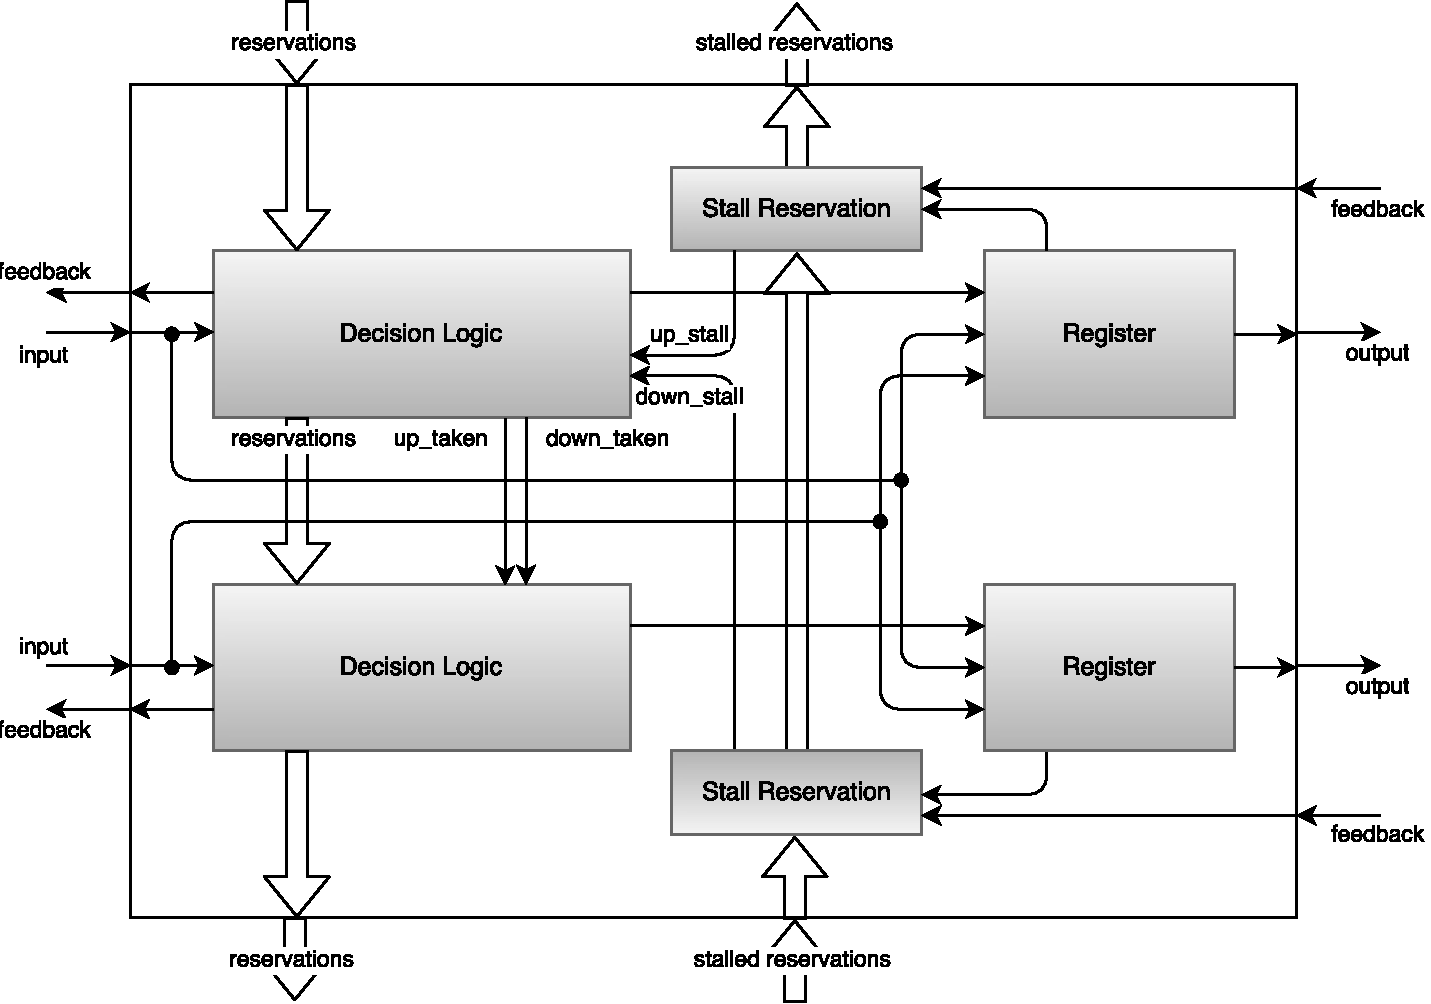
\includegraphics[width=0.8\linewidth]{benes_input_switch.pdf}
	\end{center}
\end{frame}
	
\begin{frame}
	\frametitle{Benes Network: Message Ordering}
	\begin{itemize}
		\item packet from source $s$ and destination $d$
		\item for program order of move instructions $m_n(s_n, d_n) \prec m_{n+1}(s_{n+1}, d_{n+1})$
		\item and delivery order of network $m_n \lhd m_k$
		\item input buffers require: \\
		      $(m_n(s_n, d_n) \prec m_k(s_k, d_k)) \wedge (s_n = s_k \wedge d_n = d_k)$ \\
		      $\Rightarrow (m_n(s_n, d_n) \lhd m_k(s_k, d_k))$
		
		\item Possible stalling and recursive structure $\Rightarrow$ no guarantee so far
		\item (packets with same source and destination might overtake each other)
	\end{itemize}
\end{frame}
	
